%% Submissions for peer-review must enable line-numbering
%% using the lineno option in the \documentclass command.
%%
%% Preprints and camera-ready submissions do not need
%% line numbers, and should have this option removed.
%%
%% Please note that the line numbering option requires
%% version 1.1 or newer of the wlpeerj.cls file, and
%% the corresponding author info requires v1.2

\documentclass[fleqn,10pt,lineno]{wlpeerj} % for journal submissions

% ZNK -- Adding headers for pandoc

\setlength{\emergencystretch}{3em}
\providecommand{\tightlist}{
\setlength{\itemsep}{0pt}\setlength{\parskip}{0pt}}
\usepackage{lipsum}
\usepackage[unicode=true]{hyperref}
\usepackage{longtable}


\usepackage{lipsum} \usepackage{textcomp, rotating}
\usepackage[normalem]{ulem}

\title{Detecting the impact of land cover change on observed rainfall.}

\author[1]{Chun X. Liang}

\author[1]{Floris F. van Ogtrop}

\author[1]{R. Willem Vervoort}

\corrauthor[1]{R. Willem Vervoort}{\href{mailto:willem.vervoort@sydney.edu.au}{\nolinkurl{willem.vervoort@sydney.edu.au}}}

\affil[1]{Sydney Institute of Agriculture, The University of Sydney, NSW 2006}


%
% \author[1]{First Author}
% \author[2]{Second Author}
% \affil[1]{Address of first author}
% \affil[2]{Address of second author}
% \corrauthor[1]{First Author}{f.author@email.com}

% 

\begin{abstract}
This is the supplementary data for the paper ``Detecting the impact of
land cover change on observed rainfall.'' Peerj article number 35847
% Dummy abstract text. Dummy abstract text. Dummy abstract text. Dummy abstract text. Dummy abstract text. Dummy abstract text. Dummy abstract text. Dummy abstract text. Dummy abstract text. Dummy abstract text. Dummy abstract text.
\end{abstract}

\usepackage{amsthm}
\newtheorem{theorem}{Theorem}[section]
\newtheorem{lemma}{Lemma}[section]
\theoremstyle{definition}
\newtheorem{definition}{Definition}[section]
\newtheorem{corollary}{Corollary}[section]
\newtheorem{proposition}{Proposition}[section]
\theoremstyle{definition}
\newtheorem{example}{Example}[section]
\theoremstyle{definition}
\newtheorem{exercise}{Exercise}[section]
\theoremstyle{remark}
\newtheorem*{remark}{Remark}
\newtheorem*{solution}{Solution}
\begin{document}

\flushbottom
\maketitle
\thispagestyle{empty}

\section{Code from the paper on
Github}\label{code-from-the-paper-on-github}

The Rmarkdown documents contain the code used in the analysis. These
documents including most of the data and additional scripts are
accessible via Github:
\url{https://github.com/WillemVervoort/RainfallLandcover/releases}.\\
Please cite our paper if you plan to use any of the code.

\section{Summary of Data}\label{summary-of-data}

This is a summary table of all the data used in the paper.

\begin{sidewaystable}
 \caption{Summary of data.}
  \label{tab:ch3Data}
 \begin{tabular}{lllll}
  \hline
  \textbf{Data} & \textbf{Source} & \multicolumn{2}{c}{\textbf{Resolution}} & \textbf{Analysis period} \\\cline{3-4}
  & & Temporal & Spatial & \\\hline
  Percent tree cover & MOD44B & Annual &    250m & 2000-2010\\
  Trend of vegetation cover change  &   DLCD (2009) & Onetime & 250m    & Trend of Apr 2000 - Apr 2008\\
  Rainfall &    AWAP gridded rainfall data &    Monthly &   0.05\textdegree$\times$0.05\textdegree & Jan 1979- Dec 2008\\
  SOI   & BoM   & Monthly & N/A &   Jan 1979- Dec 2008\\
  NINO 3, 3.4, 4 &  IRI/LDEO data library   & Monthly   & N/A   & Jan 1979- Dec 2008\\
  PDO   & NOAA & Monthly    & N/A   & Jan 1979- Dec 2008\\
  IOD   & POAMA-2 dataset   & Monthly   & N/A   & Jan 1979- Dec 2008\\
  \hline
  \end{tabular}
\end{sidewaystable}

\newpage

\section{Cross correlations Rainfall and Climate
Indices}\label{cross-correlations-rainfall-and-climate-indices}

These figures were moved to the supplementary data in the review
process.

\begin{figure}
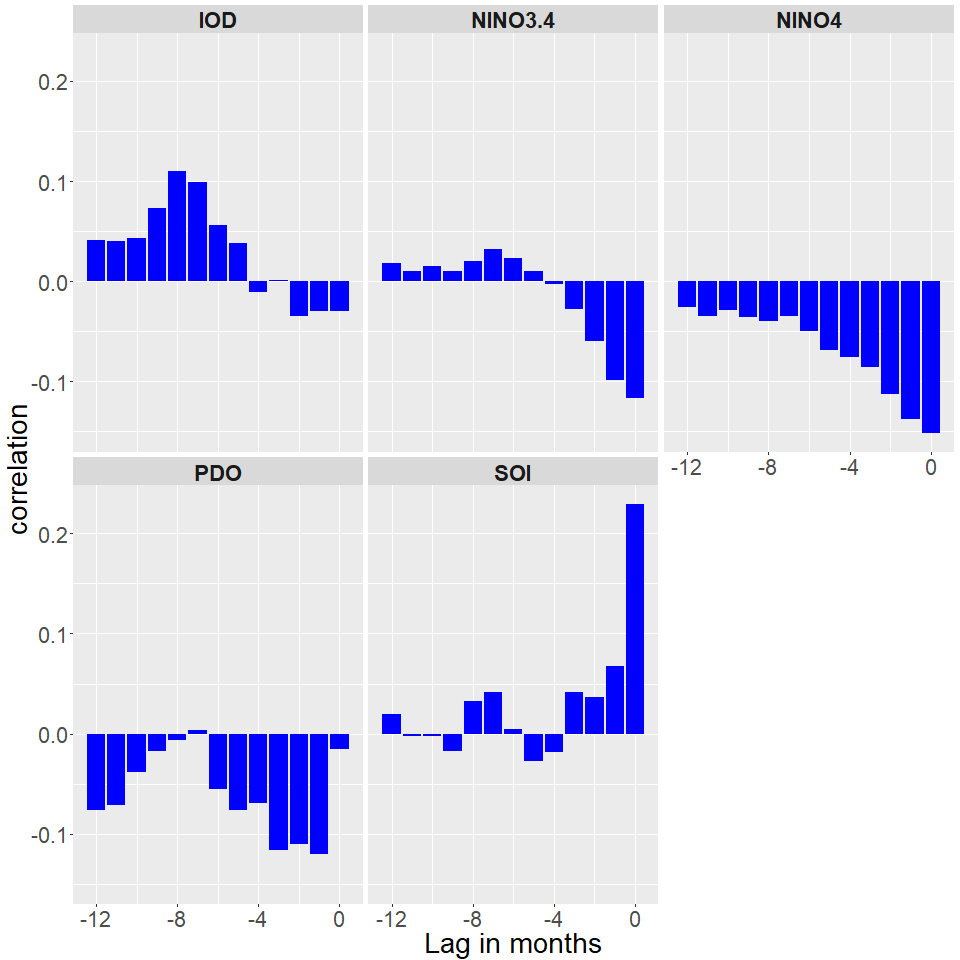
\includegraphics[width=0.9\linewidth]{figures/FigS1} \caption{Cross-correlation of six climate indices and rainfall in QLD study region. Bars in the plot indicate the strength of the cross-correlation at different lags. For the PDO analysis, 108-year rainfall data (1900 - 2008) are used. Otherwise, 36-year rainfall data are used. The correlation with NINO 3 is not shown as it is very similar to but weaker than for NINO 3.4.}\label{fig:cor-rain-qld}
\end{figure}

\begin{figure}
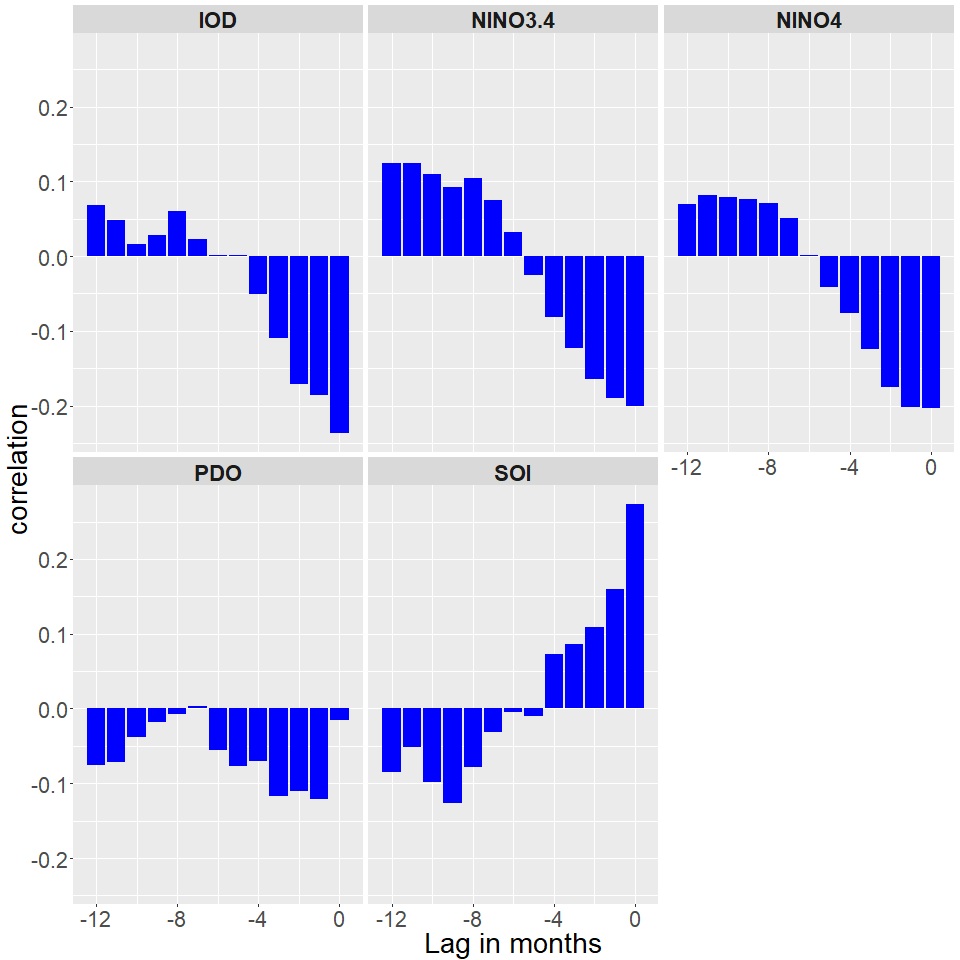
\includegraphics[width=0.9\linewidth]{figures/FigS2} \caption{Cross-correlation of six climate indices and rainfall in NSW/VIC study region. Bars in the plot indicate the strength of the cross-correlation at different lags. For the PDO analysis, 108-year rainfall data (1900 - 2008) are used. Otherwise, 36-year rainfall data are used. The correlation with NINO 3 is not shown as it is very similar to but weaker than for NINO 3.4.}\label{fig:cor-rain-nsw}
\end{figure}

Based on the correlation between the climatic indices and rainfall in
the regions (as shown in Figure \ref{fig:cor-rain-qld} and Figure
\ref{fig:cor-rain-nsw}), it can be concluded that:

\begin{itemize}
\tightlist
\item
  In QLD, the correlation between rainfall and SOI at zero time lags is
  the strongest across all indices, outweighing the other ENSO
  indicators. IOD and PDO have a weak influence in QLD.\\
\item
  In NSW/VIC, again the SOI has the strongest correlation with rainfall,
  followed by the IOD. For both, the strongest correlations occur at the
  zero time lags.\\
\item
  In both cases PDO had the weakest correlations, and this factor was
  therefore dropped as a predictor.\\
\item
  In general, for the better correlated indices, strongest correlations
  occured at zero time lags.
\end{itemize}

Although some indices are serially correlated with rainfall up to
several months, the lag zero events have the greatest correlation
coefficients. Furthermore, using multiple climatic index series was
generally found most useful in rainfall prediction (e.g. Risbey et al.
2009; Kamruzzaman, Beecham, and Metcalfe 2011).

\newpage

\section{Further figures}\label{further-figures}

These two figures highlight the GAM residual analysis for a sample
pixel. Residuals for other pixels were similar across the regions
analysed.

\begin{figure}
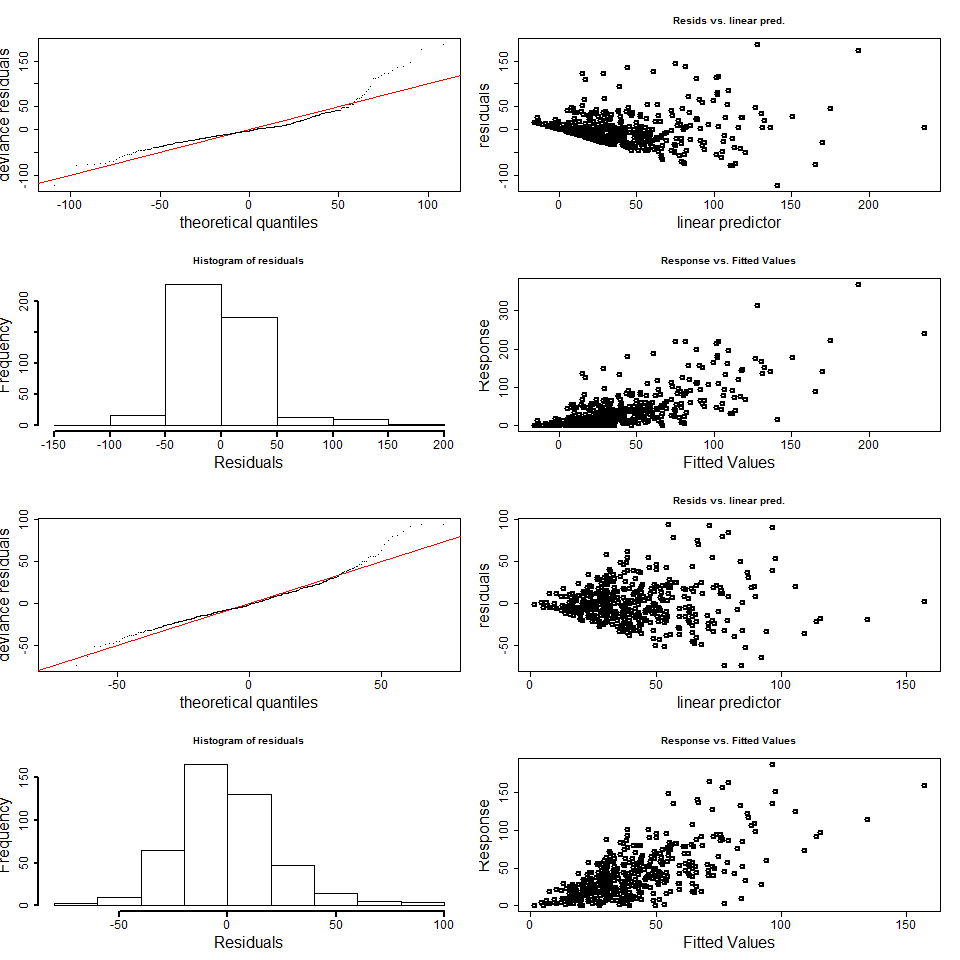
\includegraphics[width=0.9\linewidth]{figures/FigS3} \caption{The residual analysis of the Generalised additive modelling  indicating how well the residuals follow the regression assumptions. Results are shown for a sample pixel in the QLD region (top) and NSW/VIC region (bottom). Residuals are fairly normal as seen from the histogram and the qqplot, but show some scattering in the variance.}\label{fig:residuals}
\end{figure}

This figure indicates a boxplot of the annual rainfall residuals across
the regions.

\begin{figure}
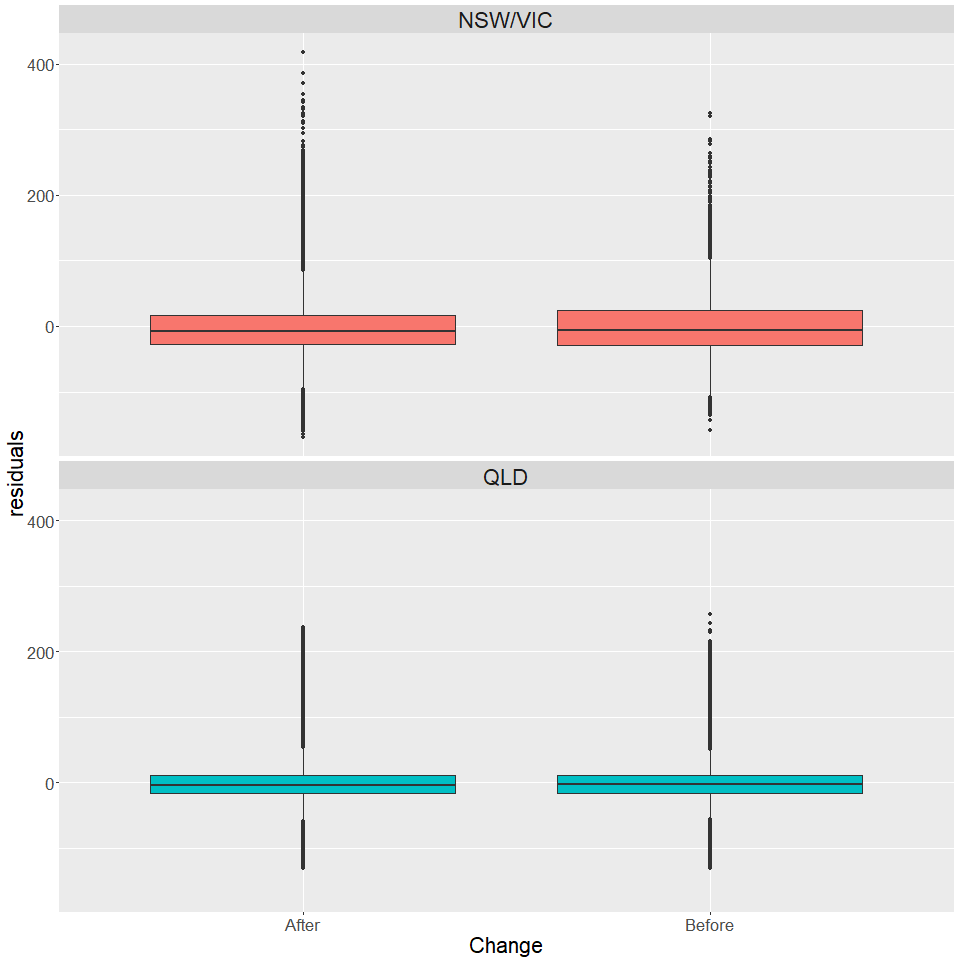
\includegraphics[width=0.7\linewidth]{figures/FigS4} \caption{Boxplots of annual rainfall residuals (estimated based on Equation 2 before and after the land cover intervention during 1979 - 2015 in the study regions. On average, the after period has a significantly lower annual rainfall residual in NSW/VIC, but a significantly higher annual rainfall residual in the Qld study area}\label{fig:meandiff}
\end{figure}

\section*{References}\label{references}
\addcontentsline{toc}{section}{References}

\hypertarget{refs}{}
\hypertarget{ref-Kamruzzaman2011}{}
Kamruzzaman, M., S. Beecham, and A. V. Metcalfe. 2011.
``Non-Stationarity in Rainfall and Temperature in the Murray Darling
Basin.'' \emph{Hydrological Processes} 25 (10). John Wiley \& Sons,
Ltd.: 1659--75. \url{http://dx.doi.org/10.1002/hyp.7928}.

\hypertarget{ref-Risbey2009}{}
Risbey, James S., Michael J. Pook, Peter C. McIntosh, Matthew C.
Wheeler, and Harry H. Hendon. 2009. ``On the Remote Drivers of Rainfall
Variability in Australia.'' \emph{Monthly Weather Review} 137 (10):
3233--53. \url{http://dx.doi.org/10.1175/2009MWR2861.1}.



\end{document}
